\documentclass[11pt,a4paper]{article}
\usepackage[margin=24mm]{geometry}
\usepackage[T1]{fontenc}
\usepackage{lmodern,microtype,amsmath,amssymb,amsthm,graphicx,booktabs,tabularx}
\usepackage[font=small,labelfont=bf]{caption}
\usepackage[numbers,sort&compress]{natbib}
\usepackage{xcolor}
\definecolor{ink}{HTML}{173E4C}
\usepackage[colorlinks=true,linkcolor=ink,citecolor=ink,urlcolor=ink,breaklinks=true]{hyperref}
\usepackage{url,fancyhdr}
\pagestyle{fancy}\fancyhf{}\fancyhead[L]{\small Oracle headroom and seed transfer}\fancyhead[R]{\small Research manuscript}\fancyfoot[C]{\thepage}
\setlength{\headheight}{14pt}
\setlength{\emergencystretch}{2em}
\newtheorem{proposition}{Proposition}
\newcommand{\E}{\mathbb{E}}
\newcommand{\Prob}{\mathbb{P}}
\newcommand{\ind}{\mathbf{1}}
\newcommand{\pp}{\,\mathrm{pp}}
\makeatletter
\newcommand{\tablerows}[1]{\@@input #1 }
\makeatother
\title{\textbf{Oracle Headroom Is Policy-Dependent:}\\A Seed-Transfer Audit of Early-Exit Networks}
\author{}
\date{}
\begin{document}
\maketitle
\begin{abstract}
Early-exit networks offer several predictions at different computational costs. A label-informed oracle measures the accuracy available among these predictions, but its relationship to transferable routing is less direct. We investigate that relationship using public per-example predictions from 45 CIFAR-100 models spanning 15 architectures and three training seeds, with complementary joint-training and multi-scale experiments. We distinguish prediction complementarity, budget-constrained oracle accuracy, transfer of an oracle policy between seeds, and held-out learned routing. For binary correctness and ordered exit costs, we implement an exact randomized budget oracle and characterize the range of target-seed accuracies attainable by source-optimal policies. Three findings change the interpretation of oracle headroom. First, resolving tied allocations improves the median same-seed oracle by 7.88 percentage points at a normalized prefix-cost budget of 0.50 relative to the original deterministic solver. Second, at budget 0.80, a canonical transferred policy is 7.43 points below confidence under a common budget cap, but 14.20 points above confidence at matched realized cost. Third, source-optimal policies at that budget span a median target-accuracy interval of 25.78 points. Thus, a single transferred-oracle score is sensitive to both policy selection and resource accounting. A separate router-fitting, calibration, and evaluation split yields only a 0.18-point median gain for a transferred confidence-feature logistic gate at target budget 0.80, with a descriptive architecture-resampling interval that includes zero. We provide an auditable evaluation protocol and reproducible analysis that preserve the oracle's role as an upper bound without interpreting seed transfer as a deployable ceiling or an estimate of pure noise.
\end{abstract}
\noindent\textbf{Keywords:} early exiting; adaptive inference; oracle evaluation; seed transfer; budget allocation; reproducibility

\section{Introduction}
Adaptive inference allocates computation according to the input. In an early-exit network, a prediction may be returned from an intermediate classifier instead of executing the full backbone. Branch classifiers, multi-scale feature propagation, and learned scheduling offer different ways to improve the resulting accuracy--cost trade-off \citep{branchynet,msdnet,eenet}. The practical motivation is straightforward: inputs need not benefit equally from additional computation. The evaluation problem is subtler, because an intermediate prediction may be correct even when the final prediction is wrong.

A common diagnostic asks what accuracy would be obtained if the evaluator could select a correct exit whenever one exists. This correctness oracle is a legitimate upper bound over the available exit predictions. However, it uses the true label, ignores the difficulty of recognizing a useful exit online, and may leave many equally optimal choices unspecified. Transferring its selected exit indices from one trained model to another removes direct optimization against the target model's correctness pattern, but it does not remove label information. Nor does source-seed optimality uniquely determine how a policy behaves on the target seed.

These distinctions matter empirically. In the atlas examined here, a deterministic budget solver makes whole groups of examples switch exits at the same Lagrange multiplier. Returning only the feasible side of such a switch can leave avoidable budget slack. Once all source-correct examples have been recovered, a minimum-cost oracle leaves additional budget unused by design. A confidence rule may continue spending that budget and increasing its accuracy. Comparing these policies at the same budget cap therefore answers a different question from comparing them at the same realized cost. Neither comparison is intrinsically invalid; the problem is treating their conclusions as interchangeable.

We study this problem through a revision-pinned reanalysis of an existing public experiment collection. The main dataset contains 45 independently trained models within 15 architecture--recipe combinations, with three seeds per architecture. Their shared CIFAR-100 evaluation examples permit 90 ordered, within-architecture seed transfers. Additional experiments establish that prediction complementarity survives joint exit training, a custom ImageNet-100 setting, and a documented MSDNet variant. These controls motivate the routing question but do not establish the learnability of every recoverable prediction.

Our contribution is an evaluation study with three components. First, we apply an information hierarchy that separates correctness complementarity, source-oracle optimization, target-seed transfer, and sequential learned routing. The broader distinction between oracle opportunity and realizability is already explicit in recent routing diagnostics \citep{selection,routingnoise}. Here we give an exact allocation construction for the binary-correctness setting and a linear program that measures selection sensitivity among source-optimal policies. The construction is a specialization of elementary resource allocation, not a new general-purpose optimization algorithm. Second, we quantify how tied allocations, realized cost, and source-policy selection affect conclusions across the atlas. Third, we replace a previously overlapping router evaluation with a disjoint fit/calibration/evaluation analysis and release the resulting tables, manifests, and figure code.

The principal result is not that oracles are invalid or that early-exit gains are unattainable. It is that \emph{oracle headroom does not identify a unique transferable routing opportunity}. At budget 0.80, the canonical transferred oracle spends a median normalized cost of 0.496. Its median advantage over confidence changes from $-7.43\pp$ under a common budget cap to $+14.20\pp$ under matched realized cost. Moreover, policies with the same optimal source accuracy permit a median $25.78\pp$ range of target accuracies. These are properties of the evaluation problem itself, before choosing a trainable router.

\section{Related work}
\paragraph{Adaptive depth and early exits.}
BranchyNet introduced side branches that permit confidence-dependent early inference \citep{branchynet}. MSDNet explicitly addresses resource-limited classification using multi-scale features and multiple classifiers \citep{msdnet}. Early-exit design and deployment are reviewed by \citet{adaptive} and \citet{survey}, while \citet{dynamic} place input-dependent computation in the broader context of dynamic networks. Our work operates on saved exit predictions and does not introduce a backbone, branch architecture, or runtime scheduler. Its focus is the interpretation of an oracle used to evaluate such systems.

\paragraph{Overthinking and example difficulty.}
\citet{overthinking} distinguish wasteful computation from destructive overthinking, in which an initially correct prediction becomes incorrect deeper in a network. The complementarity identity used below is a direct formalization of this already established phenomenon. It is not our novelty claim. Prediction depth also connects intermediate representations with example difficulty, uncertainty, and learning dynamics \citep{difficulty}. Our analysis concerns correctness at attached exit classifiers; it should not be conflated with a general, architecture-independent notion of intrinsic example difficulty.

\paragraph{Learned and consistency-based routing.}
EENet learns an early-exit scheduler subject to an average inference budget \citep{eenet}. PTEENet studies post-trained branches attached to pretrained networks \citep{pteenet}. Patience-based early exiting uses repeated prediction agreement as a stopping signal in language models \citep{patience}. These methods establish that router design is substantive and that richer policies can exploit signals unavailable to a scalar threshold. Our logistic gate is deliberately restricted to exit-local confidence features. It is a diagnostic baseline, not a reproduction of these methods or a competitive state-of-the-art router comparison.

\paragraph{Calibration and computational accounting.}
Softmax confidence need not equal correctness probability \citep{calibration}. In this manuscript, \emph{budget calibration} means choosing a threshold to satisfy an average cost constraint on a separate input set; it does not mean probability calibration or a statistical risk guarantee. Likewise, theoretical operation counts differ from device latency because memory access and platform characteristics matter \citep{shuffle}. We report normalized backbone-prefix-plus-head operation counts, explicitly excluding some sequential overhead, and make no measured latency or energy claim.

\paragraph{Recent oracle-gap diagnostics.}
\citet{selection} separate outcome-oracle opportunity, signal-restricted opportunity, and held-out learned-router gain for multi-LLM routing, and develop inference that accounts for baseline and policy selection. \citet{routingnoise} analyze how stochastic decoding can inflate a single-draw routing oracle relative to reproducible specialist advantage. These studies directly caution against interpreting an oracle gap as learnable gain. Our fixed exit-prediction setting varies trained classifier seeds rather than decoding draws, so their stochastic-noise decomposition is not automatically applicable. Our additional focus is the interaction between discrete budget allocation, realized cost, and non-unique source-optimal policies. We do not provide the selection-valid population guarantees of \citet{selection}; our architecture bootstrap is explicitly conditional and descriptive.

These lines of work motivate a narrower contribution than a new early-exit method: an executable audit of which oracle quantity is being reported, how an optimal policy is selected, and whether its apparent advantage survives changes in the comparison protocol. We do not claim priority for overthinking, fractional allocation, or the general distinction between oracle opportunity and realizability.

\section{What an early-exit oracle measures}
\subsection{Predictions, policies, and information access}
Let $s$ index a training seed, $i\in\{1,\ldots,n\}$ index an aligned example, and $k\in\{1,\ldots,K\}$ index an exit. Define
\begin{equation}
 c^{s}_{ik}=\ind\{\widehat y^{s}_{ik}=y_i\}, \qquad
 0<r_1<\cdots<r_K=1,
\end{equation}
where $r_k$ is a normalized cost shared by seeds of one architecture. A randomized policy is represented offline by $\pi_{ik}\geq0$, with $\sum_k\pi_{ik}=1$. Its target-seed accuracy and expected cost are
\begin{equation}
 A_t(\pi)=\frac1n\sum_{i,k}\pi_{ik}c^t_{ik},\qquad
 R(\pi)=\frac1n\sum_{i,k}\pi_{ik}r_k.
 \label{eq:policy}
\end{equation}
The oracle may inspect all correctness indicators. A deployable sequential policy may inspect only signals available up to the current exit, without $y_i$. A transferred oracle retains the source-seed labels and predictions; it is a retrospective diagnostic evaluated on the same aligned images.

\begin{table}[t]
\centering\small
\caption{The information hierarchy. ``Target labels'' refers to their use in selecting an exit, not their routine use in scoring accuracy.}
\begin{tabularx}{\linewidth}{@{}lXX@{}}
\toprule
Quantity & Exit-selection information & Interpretation \\
\midrule
Any-correct-exit accuracy & All target exits and labels & Prediction complementarity; no budget constraint \\
Budget oracle & All target exits and labels & Upper bound over the recorded predictions and cost model \\
Transferred oracle & All source exits and labels for the evaluation images & Behavior of a specified source-optimal policy on a target seed \\
Held-out sequential gate & Current-exit signals; fitted on other images & Performance of one deployable-form rule under the recorded cost model \\
\bottomrule
\end{tabularx}
\label{tab:hierarchy}
\end{table}

\subsection{Complementarity is an exact set identity}
Define the any-correct-exit and final-exit accuracies as
\begin{equation}
 U_s=\frac1n\sum_i\max_k c^s_{ik},\qquad F_s=\frac1n\sum_i c^s_{iK}.
\end{equation}
Since the final exit belongs to the set of candidate exits,
\begin{equation}
 U_s-F_s=\frac1n\sum_i\ind\{c^s_{iK}=0,\ \max_{k<K}c^s_{ik}=1\}.
 \label{eq:identity}
\end{equation}
This difference counts examples saved by an earlier classifier. It cannot establish that those examples are unrecognizable by a learned router. A correct selector could exceed final-exit accuracy. Conversely, a large difference alone does not show that a sequential selector can identify the useful exit cheaply.

\subsection{An exact budget-constrained correctness oracle}
The same-seed oracle value at budget $b\geq r_1$ is
\begin{equation}
 O_s(b)=\max_{\pi:R(\pi)\leq b} A_s(\pi).
 \label{eq:oracle}
\end{equation}
For binary correctness and common ordered costs, the optimization has a simple allocation structure. Begin by assigning every example to exit 1. Examples already correct there cannot gain accuracy. Among examples incorrect at exit 1 but correct somewhere later, let $e_i$ be the earliest correct exit and $d_i=r_{e_i}-r_1$. Upgrading example $i$ yields one additional correct prediction at extra cost $d_i$. Examples incorrect at every exit cannot improve the source objective.

\begin{proposition}
An optimal randomized solution to Eq.~\eqref{eq:oracle} upgrades eligible examples in increasing order of $d_i$. At the boundary cost, a common fractional upgrade probability over the tied group achieves the optimum. If every eligible example is upgraded, the remaining budget may be left unused.
\end{proposition}
\begin{proof}
Any source-incorrect allocation is weakly dominated, for source accuracy and cost, by exit 1. Any source-correct allocation is weakly dominated by the earliest source-correct exit. Thus only the binary upgrades above remain. If a higher-cost upgrade has positive allocation while a lower-cost one is not fully allocated, exchanging equal upgrade probability preserves accuracy and weakly reduces cost. Repeating this exchange yields increasing-cost allocation. A fractional final group spends the remaining useful budget exactly. Once all upgrades are allocated, the any-correct-exit value is attained and cannot be improved.
\end{proof}

Our \emph{canonical policy} uses exit 1 for examples with no source-correct exit and uses a uniform probability within a boundary group. This specifies behavior that source accuracy alone leaves ambiguous. The reported accuracy and cost integrate over this randomization exactly; we do not draw stochastic routing outcomes. The budget is an expected average, not a hard constraint on every randomized batch realization.

The original solver instead selected $\arg\max_k(c^s_{ik}-\lambda r_k)$ and bisected on $\lambda$, retaining the feasible side. All examples with the same earliest-correct exit have the same upgrade cost, so they may change decisions together. Bisection does not by itself interpolate across that discontinuity. It can therefore return a feasible but suboptimal accuracy. Our implementation is checked against 30 independently formulated linear programs on randomized small instances.

\subsection{Source-optimality does not identify target accuracy}
For source $s$ and target $t$, let $\pi^\star_s(b)$ denote the canonical source-optimal policy. Its transfer score is
\begin{equation}
 T_{s\rightarrow t}(b)=A_t(\pi^\star_s(b)).
\end{equation}
The paired difference $O_t(b)-T_{s\rightarrow t}(b)$ is a \emph{seed-transfer gap}. It includes source--target disagreement and policy selection effects; it is not automatically statistical bias or irreducible noise.

More fundamentally, define the full source-optimal policy set
\begin{equation}
 \Pi_s^\star(b)=\{\pi:R(\pi)\leq b,\ A_s(\pi)=O_s(b)\}.
\end{equation}
Its target-accuracy envelope is
\begin{equation}
 L_{s\rightarrow t}(b)=\min_{\pi\in\Pi_s^\star(b)}A_t(\pi),\quad
 H_{s\rightarrow t}(b)=\max_{\pi\in\Pi_s^\star(b)}A_t(\pi).
 \label{eq:envelope}
\end{equation}
Both endpoints are linear programs. They use target labels and are \emph{sensitivity bounds}, not algorithms available at deployment. A wide interval demonstrates that source optimality and the budget cap are insufficient to determine a transferred-oracle score.

For example, when every source exit is incorrect for an input, routing it deeper does not change source accuracy. If a deeper target exit is correct, the same choice changes target accuracy. A source-optimal policy can exploit spare budget on such cases without losing source accuracy. Even without all-incorrect cases, several source-correct exits can disagree on the target. Our canonical minimum-cost convention resolves these choices, but it does not make their consequences intrinsic properties of the target model.

\subsection{Common caps and matched realized costs}
Let $B_t(b)$ be the accuracy of a target confidence rule calibrated to the largest feasible threshold at cost cap $b$. We distinguish
\begin{align}
 D_{\mathrm{cap}}(b)&=T_{s\rightarrow t}(b)-B_t(b),\\
 D_{\mathrm{cost}}(b)&=T_{s\rightarrow t}(b)-B_t(R(\pi_s^\star(b))).
 \label{eq:comparison}
\end{align}
The first compares feasible policies offered the same allowance. The second compares them at approximately equal realized cost. In the retrospective oracle audit, confidence thresholds use the evaluation inputs to match cost without using their labels; we call this \emph{transductive cost matching}. It is not the held-out deployment protocol used for the learned gates below. Discrete confidence ties can leave a small discrepancy, which we report explicitly.

\section{Experimental design and provenance}
\subsection{Frozen atlas and supplementary training regimes}
The main atlas comprises CIFAR-100 \citep{cifar} models with $32\times32$ inputs: five residual variants, three wide residual networks, two VGG variants, MobileNetV2, ShuffleNetV2, ConvNeXt-Femto, ViT-Tiny, and Mixer-Nano. These span residual \citep{resnet,wide}, convolutional \citep{vgg,mobile,shuffle,convnext}, attention \citep{vit}, and MLP \citep{mixer} families. These are the project's implementations and recipes, not uniformly reproduced published reference models. Each architecture has seeds 1--3. The backbone is trained first and attached exits are then fitted with the backbone frozen. Fourteen architectures have five distinct exits; ResNet8x4 has three, as listed in Appendix~\ref{app:atlas}.

The CIFAR-100 training set contains 50,000 images and the test set 10,000. We use all 10,000 aligned test predictions for the oracle and complementarity analyses. The 90 ordered source--target pairs are obtained from 45 models; they are not 90 independent training runs. The analysis checks unique sample identifiers and identical ordered labels across all models, rather than truncating arrays to a common length.

The archived seed-1 configurations use 240 backbone epochs for the conventional convolutional models, with SGD, initial learning rate 0.05, batch size 64, weight decay $5\times10^{-4}$, and learning-rate drops at epochs 150, 180, and 210. ConvNeXt-Femto, Mixer-Nano, and ViT-Tiny use 300 epochs with AdamW, initial learning rate 0.001, batch size 128, weight decay 0.05, and cosine scheduling. All archived seed-1 frozen configurations specify 20 exit-fitting epochs with exit learning rate 0.01. These recipe differences are part of the atlas, so an architecture contrast is not a controlled intervention on architecture alone.

Three joint-training controls use ResNet20, ResNet32x4, and VGG8 on CIFAR-100, with one joint seed each. Two further joint models use ResNet50 and ViT-S/16 on a custom ImageNet-100 subset derived from ImageNet \citep{imagenet}. The subset takes the first 100 sorted WordNet identifiers, producing an animal-heavy class selection rather than a random or canonical ImageNet-100 benchmark. It contains 119,395 training and 10,000 evaluation images, with 100 evaluation examples per class, at $224\times224$ resolution. Its 15,000-image training diagnostic slice is drawn from training data and is not an independent validation set. The cross-dataset controls support the existence of complementarity in this setting, not a causal estimate of a dataset-scale effect.

Finally, two jointly trained MSDNet-variant seeds provide a multi-scale control. The variant has three scales, 20 layers, base width 16, growth rate 6, and exits at layers 4, 8, 12, 16, and 20. It omits the original model's bottleneck and channel-reduction transitions and uses linear exit classifiers. It has 1,521,336 training parameters. These choices preclude describing it as an official MSDNet replication. Both seeds complete 240 epochs. Their recorded total training times sum to 6.941 hours on an RTX 4000 Ada; this is a historical training total, not a measurement of routing efficiency.

\subsection{Costs and scope of the resource claim}
Each architecture has a pinned cost table measured with a two-FLOPs-per-multiply-accumulate convention. A depth cost is the backbone prefix plus that exit's linear head, divided by the corresponding final-exit cost. The tables do not accumulate the costs of all previously evaluated exit heads, gate evaluation, routing control flow, or device-specific execution overhead. Our results therefore concern this \emph{prefix-cost proxy}. They are not end-to-end latency savings or complete sequential FLOP accounting. All within-architecture seed comparisons use the same cost table, and all tables are strictly increasing with final normalized cost one.

\subsection{A disjoint router evaluation}
We perform a new post-hoc routing experiment on the saved CIFAR-100 test predictions. Within each class, a fixed pseudorandom partition assigns 40 examples to fitting, 20 to calibration, and 40 to evaluation: 4,000/2,000/4,000 images in total. The partition is shared across seeds and architectures and is distributed explicitly with the analysis. No image used to fit a gate or calibrate its threshold appears in the new router evaluation set.

For each early exit, a logistic model predicts correctness from five current-exit features: the largest probability $p_1$, the second-largest $p_2$, their margin, $\log p_1$, and $p_1/p_2$. Probabilities are clipped only where necessary for the logarithm and ratio. Features are standardized using the fit subset. The logistic model uses $L_2$ regularization, $C=1$, and a 2,000-iteration limit. These settings and the split were fixed for this analysis; no hyperparameter search on the evaluation subset was performed. The same-seed gate is fitted on its target model; the transferred gate is fitted on another seed's fit images and applied to target-seed features.

At inference, the rule exits at the first predicted correctness probability at least as large as a shared threshold, otherwise using the final exit. Confidence and margin use the same sequential stopping form. For every rule, threshold selection uses only the 2,000 target calibration inputs and the cost table. Accuracy is then scored on the 4,000 evaluation inputs. We evaluate seven calibration targets: 0.40, 0.50, 0.60, 0.70, 0.80, 0.90, and 0.95. Realized evaluation cost can differ from its calibration target; both costs are retained.

This split corrects router-level image overlap, but it does not retroactively create a pristine benchmark. The underlying experiments and model selection predate this analysis, and the test set has already informed project decisions. The held-out claim is therefore conditional on these fitted models and the newly separated router stages. It is not an untouched external validation study.

\subsection{Aggregation, uncertainty, and audit boundaries}
Our primary aggregation first averages all available within-architecture seed pairs, then takes the median over 15 architectures. For a single-model quantity, we average the three seeds before taking that median. Paired differences are computed before aggregation; separately reported medians need not subtract. Bootstrap intervals use 10,000 resamples of complete architecture summaries. They describe sensitivity to the composition of this atlas, conditional on its shared examples and training runs. They do not capture new-dataset variation or establish a population of independent architecture draws. Architecture-level values and all seed-pair rows are available for inspection.

The prediction snapshot is pinned to Hugging Face revision \texttt{a6356f6a8dee} of \path{Shanmuk4622/msc-cifar100}, retrieved during the September 7--8, 2026 audit. The companion ImageNet repository is pinned separately in the evidence manifest. The two ImageNet joint controls and the MSDNet runs are stored in the CIFAR-named repository; dataset names are taken from run metadata rather than inferred from the repository name. Public source artifacts remain unchanged. The new exact-oracle, envelope, and disjoint-router results are retrospective analyses, not preregistered confirmatory experiments.

\section{Results}
\subsection{Complementarity survives changes in exit training}
Across the 45 frozen atlas models, the early-save advantage ranges from $4.81$ to $11.56\pp$. The median over individual models is $6.86\pp$; the primary median over architecture seed means is $6.72\pp$. All models exhibit some examples for which an intermediate classifier is correct and the final exit is incorrect (Fig.~\ref{fig:complementarity}). This establishes a broad empirical motivation for routing among exits, while leaving accessibility unresolved.

\begin{figure}[t]
\centering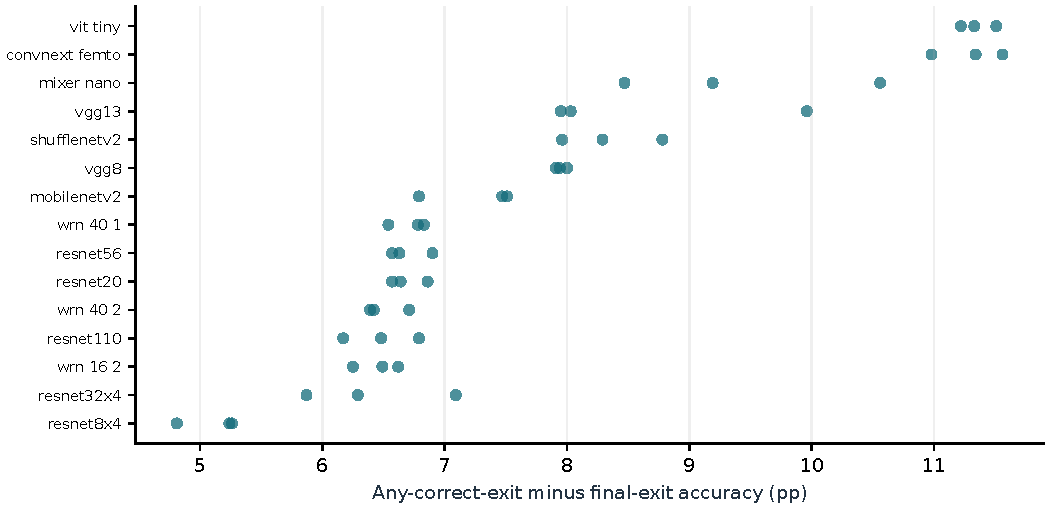
\includegraphics[width=.94\linewidth]{figures/complementarity.pdf}
\caption{Prediction complementarity in the frozen CIFAR-100 atlas. Each point is one training seed; coincident values may overlap. The horizontal coordinate is exactly the early-save fraction in Eq.~\eqref{eq:identity}, expressed in percentage points.}
\label{fig:complementarity}
\end{figure}

\begin{table}[t]
\centering\small
\caption{Supplementary joint-training controls. Accuracy is recomputed from saved depth predictions. Each row has 10,000 evaluation examples. Intervals for the three attached-exit CIFAR controls are sample-bootstrap intervals conditional on one trained model, not seed intervals.}
\begin{tabular}{@{}llrrrr@{}}
\toprule
Dataset & Model & Seed & Final (\%) & Any exit (\%) & Save (pp) \\
\midrule
CIFAR-100 & ResNet20 & 1 & 68.02 & 78.66 & 10.64 \\
CIFAR-100 & ResNet32x4 & 1 & 77.83 & 86.38 & 8.55 \\
CIFAR-100 & VGG8 & 1 & 72.28 & 81.43 & 9.15 \\
ImageNet-100 & ResNet50 & 1 & 81.58 & 88.97 & 7.39 \\
ImageNet-100 & ViT-S/16 & 1 & 63.23 & 70.14 & 6.91 \\
CIFAR-100 & MSDNet variant & 1 & 73.93 & 81.67 & 7.74 \\
CIFAR-100 & MSDNet variant & 2 & 74.08 & 81.99 & 7.91 \\
\bottomrule
\end{tabular}
\label{tab:controls}
\end{table}

Jointly training attached classifiers also preserves complementarity (Table~\ref{tab:controls}). The respective early-save advantages are $10.64$, $8.55$, and $9.15\pp$, with sample-bootstrap 95\% intervals of $[10.00,11.28]$, $[7.98,9.10]$, and $[8.61,9.71]\pp$. The custom ImageNet-100 controls yield $7.39\pp$ for ResNet50 and $6.91\pp$ for ViT-S/16. The two MSDNet-variant seeds yield $7.74$ and $7.91\pp$, averaging $7.825\pp$. Thus the phenomenon is not confined to frozen auxiliary heads in these experiments. The limited seeds and custom architectures prevent a stronger claim of architecture independence.

\subsection{Tied budget allocations materially affect oracle accuracy}
The exact randomized oracle improves the original deterministic value in 122 of the 630 ordered-pair/budget rows. Same-seed values are duplicated across source pairs in that count; it is not a count of independent improvements. At budget 0.40, the median within-architecture accuracy improvement is $7.25\pp$; at 0.50 it is $7.88\pp$. The largest individual row difference is $24.61\pp$. The median improvement is zero from 0.60 onward, although a zero median does not imply every architecture is unchanged.

\begin{figure}[t]
\centering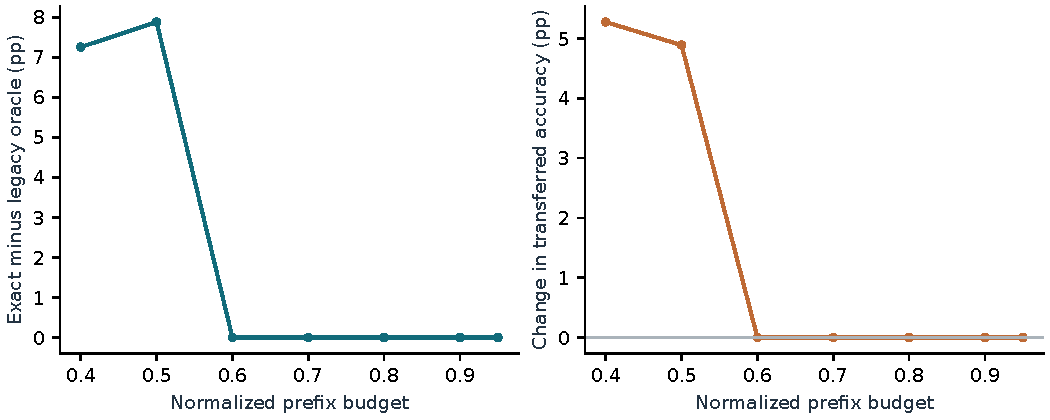
\includegraphics[width=\linewidth]{figures/solver_audit.pdf}
\caption{Effect of replacing the deterministic feasible-side Lagrange solver with exact fractional allocation. Values are medians over architecture means of paired differences. Improving the source allocation also changes the transferred score. A zero aggregate difference at a budget need not mean every run is unchanged.}
\label{fig:solver}
\end{figure}

At budget 0.50, the median avoidable cost difference between exact and legacy policies is 0.064 of the final-prefix cost. This is distinct from the \emph{unavoidable lack of useful source upgrades} after the any-correct-exit value is attained. Both produce slack, but only the former is a solver deficiency. Resolving the tied allocations increases transferred accuracy by a median $4.89\pp$ at 0.50. Consequently, an apparent limitation of seed transfer can partly reflect the source optimization implementation rather than instability of predictions.

\subsection{The budget-dependent sign reversal does not survive cost matching}
Table~\ref{tab:budgets} reports the exact canonical oracle audit. At the common 0.80 cap, the same-seed oracle has median accuracy 77.57\%, and the transferred policy 54.55\%. Their paired seed-transfer gap is $22.47\pp$. This is a substantial descriptive difference, but the transferred policy's median realized cost is only 0.496. Confidence calibrated near the full 0.80 allowance is therefore being offered more realized computation.

\begin{table}[t]
\centering\small
\caption{Exact-oracle audit on all 10,000 CIFAR-100 test examples. Accuracy columns are percentages. $D_{\mathrm{cap}}$ and $D_{\mathrm{cost}}$ are paired transfer-minus-confidence differences in percentage points. $N^+_{\mathrm{cap}}$ and $N^+_{\mathrm{cost}}$ count architectures with positive differences under each comparison, out of 15. Accuracy, cost and difference summaries are medians of architecture means; these medians need not subtract.}
\begin{tabular}{@{}rrrrrrrr@{}}
\toprule
Cap & Oracle & Transfer & Transfer cost & $D_{\mathrm{cap}}$ & $D_{\mathrm{cost}}$ & $N^+_{\mathrm{cap}}$ & $N^+_{\mathrm{cost}}$ \\
\midrule
\tablerows{budget_rows.tex}
\bottomrule
\end{tabular}
\label{tab:budgets}
\end{table}

\begin{figure}[t]
\centering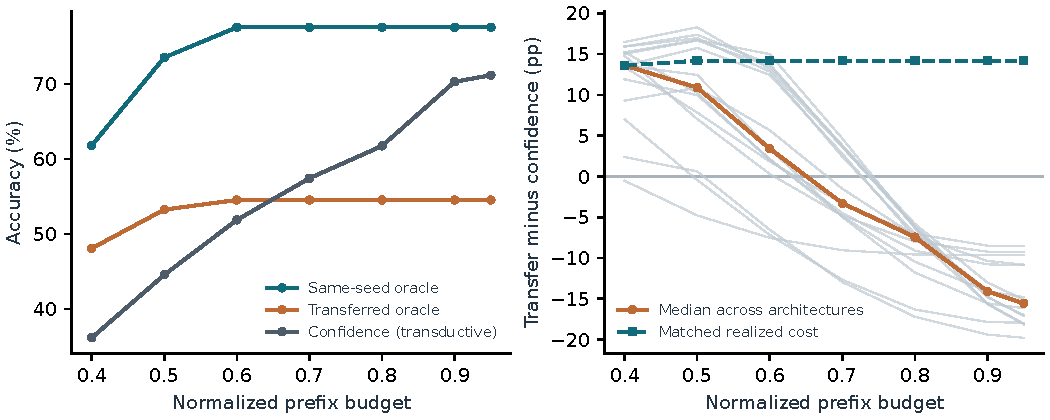
\includegraphics[width=\linewidth]{figures/budget_transfer.pdf}
\caption{Oracle transfer depends on the comparison protocol. Left: same-seed, canonical transferred-oracle, and transductively cost-calibrated confidence accuracies under a common cap. Right: cap-matched architecture differences (thin gray curves), their median (solid orange), and the median at matched realized cost (dashed teal). The transferred policy saturates before using large budgets. Neither oracle curve describes deployable routing.}
\label{fig:budgets}
\end{figure}

Under the common-cap comparison, the median transfer advantage is positive through 0.60 and negative from 0.70 onward. At 0.80 it is $-7.43\pp$, and no architecture has a positive mean advantage. Under matched realized cost, the median is instead $+14.20\pp$, with a positive difference in all 15 architectures. The corresponding architecture-resampling interval is $[11.38,16.99]\pp$. The largest confidence/oracle cost discrepancy in the matched analysis is less than $7.35\times10^{-5}$ normalized units, so the difference is not explained by a large residual cost mismatch.

The two results answer distinct questions. The common-cap result shows that the particular minimum-cost transferred policy fails to use the additional allowance productively relative to confidence. The matched-cost result shows that source correctness contains useful retrospective information at the cost this policy actually chooses. It does not show that this information is available to an online gate. Describing either curve as the unique ``honest headroom'' would obscure those distinctions.

\subsection{Source-optimal policies permit widely different target accuracies}
At cap 0.80, the median width of the source-optimal target-accuracy envelope is $25.78\pp$, with an architecture-resampling interval of $[24.02,26.73]\pp$. Architecture mean widths range from $17.38$ to $31.74\pp$. The separately aggregated lower and upper endpoint medians are 48.90\% and 76.12\%, respectively; their difference is not the median paired width. Every canonical transfer score lies inside its corresponding envelope.

\begin{figure}[t]
\centering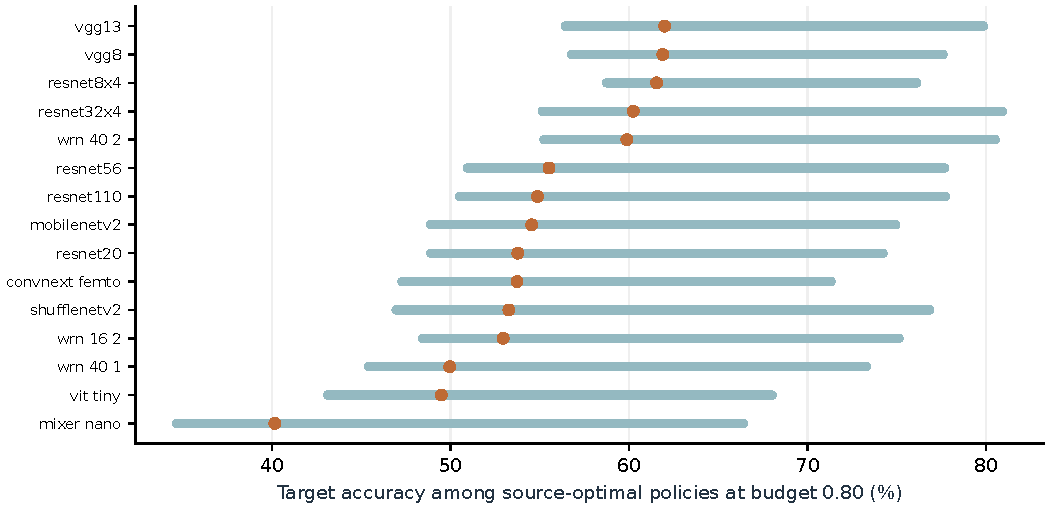
\includegraphics[width=.96\linewidth]{figures/policy_envelope.pdf}
\caption{Selection sensitivity at cap 0.80. Each horizontal interval averages the lower and upper target accuracies over the six ordered seed pairs within an architecture, while enforcing optimal source accuracy and the same cost cap. Orange points are the canonical minimum-cost transfer scores. The endpoints use target labels to diagnose non-uniqueness; they are not learned-policy performance.}
\label{fig:envelope}
\end{figure}

This interval is not a confidence interval. It is an optimization range over policies that are indistinguishable under the source accuracy objective and budget constraint. Its width provides direct evidence that a source oracle does not identify a unique target score. The envelope allows alternative policies to use spare budget; it does not hold realized cost fixed at the canonical policy's cost. Thus it combines ambiguity in exit selection with ambiguity in use of the available allowance, precisely the two freedoms left unspecified by the source-only optimization problem.

The upper endpoint is especially easy to misinterpret. It selects favorable target outcomes while preserving source optimality and therefore uses information unavailable to a transferred deployment rule. It is not evidence that a gate can attain that accuracy. Its role is to falsify an interpretation of the canonical transfer score as a target property determined by source optimality alone.

\subsection{Held-out confidence-feature routing yields modest gains}
The disjoint router analysis produces 1,575 rule/seed/budget rows. At calibration target 0.80, the median paired gain over confidence is $0.12\pp$ for same-seed logistic routing, $0.18\pp$ for transferred logistic routing, and $0.42\pp$ for margin routing. Median paired realized-cost differences are approximately $-0.00088$, $-0.00033$, and $-0.00088$, respectively. These small gains should not be equated with the much larger label-informed oracle differences.

An additional architecture-resampling check gives intervals of $[-0.04,0.36]\pp$ for the same-seed logistic gain and $[-0.02,0.40]\pp$ for the transferred logistic gain. Both include zero. The margin interval is $[0.23,0.65]\pp$. These descriptive intervals do not adjust for examining several rules or budgets and are not evidence of population-level superiority.

\begin{figure}[t]
\centering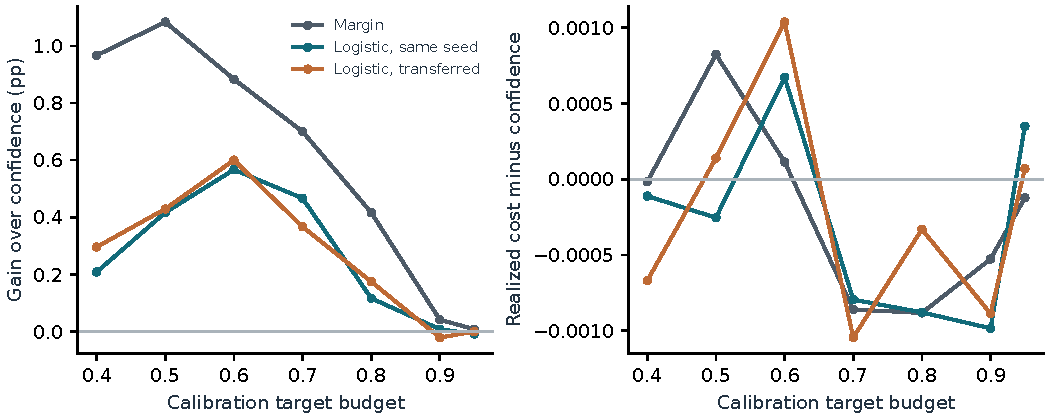
\includegraphics[width=\linewidth]{figures/heldout_routing.pdf}
\caption{Disjoint router analysis on 4,000 evaluation images after fitting on 4,000 and cost calibration on 2,000 separate images. Left: paired accuracy gain over confidence. Right: corresponding paired realized-cost difference. Each curve aggregates seed comparisons within architecture, then takes the median over architectures. Costs are close but not forced to match on the evaluation set.}
\label{fig:gate}
\end{figure}

The calibration budget is not a guaranteed test-time cap. Across all rules and budgets, 89 of 1,575 rows exceed their target by more than 0.01 normalized cost; the maximum overspend is 0.01672. Accordingly, Fig.~\ref{fig:gate} reports both accuracy and achieved cost, and we do not call these exactly budget-matched test comparisons. The oracle evaluated at each rule's realized evaluation cost is also retained in the released data.

The gate's restricted feature set and linear decision model limit what can be inferred from its small gains. It does not condition on representations or an uncertainty trajectory, and its correctness predictors are fitted independently per exit rather than on the distribution of examples that survive preceding gates. A larger or sequentially trained router could behave differently. The result establishes a concrete gap between a specified learned policy and oracle diagnostics; it does not establish that the gap is unlearnable.

\section{Discussion}
\subsection{A useful oracle needs an explicit evaluation contract}
The same-seed oracle remains mathematically useful: under its stated cost model and the same expected budget cap, no selector of the recorded exits can exceed Eq.~\eqref{eq:oracle}. A transferred source oracle has a different role. It reveals how one label-informed allocation behaves when the classifier changes, and can help study which per-example decisions persist across seeds. To interpret it, the evaluator must specify the source objective, the allocation solver, the tie rule, the treatment of source-incorrect examples, and whether a budget is a cap or a matched expenditure.

Our results show why these details are not cosmetic. An underfilled boundary group changes tight-budget oracle accuracy by several points. A minimum-cost convention leaves a large allowance unused after source accuracy saturates. Another source-optimal policy can spend that allowance differently and obtain a very different target score. A transfer curve reported without these choices combines classifier behavior with an unspecified policy-selection mechanism.

An effective reporting protocol should therefore provide five items: a precisely defined correctness objective and information set; an exact or independently validated resource-allocation solution; achieved costs alongside target budgets; sensitivity to non-unique source-optimal choices; and a separately fitted and calibrated sequential baseline. The supplied analysis implements these checks on immutable predictions. They are inexpensive relative to training the backbones and can be applied to other multi-exit evaluations with the same binary-correctness structure.

\subsection{What the controls support}
The joint-training and multi-scale controls strengthen the conclusion that final-exit accuracy is not the maximum accuracy present among available classifiers. They do not identify a universal mechanism or a bound on trainable routing. Likewise, the ImageNet subset extends the observation to a larger input resolution and different architectures, but confounds dataset, resolution, recipe, and model family. Its class selection and one-seed controls should remain visible in any comparison with other ImageNet-100 reports.

The broader project also examines cross-axis compute difficulty, softmax reliability, and data pruning. We do not combine those analyses into a causal explanation for the oracle-transfer gap. In particular, a correlation between training saturation and score reliability is not evidence that memorization causes all transfer loss, and a pruning comparison with different data pools does not establish downstream harm. Keeping the present manuscript centered on its identifiable evaluation quantities produces a more testable contribution.

\subsection{Limitations and scope}
This is a retrospective audit of a fixed, relatively small atlas. Architectures are not random draws, seeds share examples, and many models share design choices. Architecture resampling cannot repair those dependencies or establish external generalization. The new router split limits direct image reuse within the routing experiment but does not erase earlier benchmark reuse. Its results are descriptive rather than confirmatory.

Cost conclusions are limited to prefix-plus-one-head operation counts. Full sequential head costs, router costs, device measurements, and batch scheduling remain unmeasured. The transferred oracle has access to labels through the source model and cannot be deployed as reported. The envelope endpoints use additional target-label information and must not be presented as achievable routing systems. The joint and multi-scale controls are small and use project-specific implementations. A generic final-evaluation artifact in those joint runs also scores an inactive backbone classifier; we quarantine that artifact and use the verified trained depth heads instead, as detailed in Appendix~\ref{app:provenance}.

There is no direct experimental comparison with strong modern learned routers, an official MSDNet reproduction, or an external test dataset. Those additions would strengthen the manuscript as a broad empirical early-exit study. The present evidence supports a methodological evaluation contribution: oracle optimization, policy selection, and realized cost can materially change the conclusions drawn from a fixed set of predictions.

\section{Conclusion}
Early-exit oracle accuracy, seed-transfer accuracy, and learned routing performance are distinct measurements. In a 45-model CIFAR-100 atlas, exact tied-budget allocation substantially changes tight-budget oracle values; matched realized cost reverses the interpretation of a common-cap transfer deficit; and source-optimal policies admit a wide range of target accuracies. Complementary joint and multi-scale experiments verify that useful intermediate predictions exist, while a disjoint confidence-feature gate experiment shows that their existence alone does not imply a large gain for a simple learned router. These findings support reporting oracle values together with their optimization, policy-selection, cost, and information-access assumptions. Doing so preserves the diagnostic value of oracles while avoiding claims about deployable headroom that the measurements do not identify.

\section*{Data and code availability}
Public experiment artifacts are available at \url{https://huggingface.co/datasets/Shanmuk4622/msc-cifar100} and \url{https://huggingface.co/datasets/Shanmuk4622/msc-imagenet100}. The accompanying source package contains the analysis scripts, figure inputs, the explicit router split, input hashes and revision-pinned URLs, and the bibliography verification record. Large prediction files can be retrieved using the input manifest; no access token is required. The public artifact repositories are cited for reproducibility and do not imply permission to redistribute underlying ImageNet images outside their original terms.

\appendix
\section{Architecture-level atlas results}\label{app:atlas}
\begin{table}[h]
\centering\small
\caption{Frozen CIFAR-100 atlas. Accuracy and early-save values are means over three seeds, recomputed from exit predictions. Parameter counts describe the archived backbone summary and are rounded; they do not include all routing overhead.}
\begin{tabular}{@{}lrrrrr@{}}
\toprule
Architecture & Exits & Params (M) & Final (\%) & Any exit (\%) & Save (pp) \\
\midrule
\tablerows{atlas_rows.tex}
\bottomrule
\end{tabular}
\end{table}

\section{Optimization and reproducibility details}
The exact solver begins with $nr_1$ cost and the number of correct first-exit predictions. For a nonempty group $G_k=\{i:c^s_{i1}=0,e_i=k\}$, the extra cost is $|G_k|(r_k-r_1)$ and the accuracy gain is $|G_k|/n$. Empty groups are skipped. Groups are processed in ascending exit order. If remaining budget is $B$, the group upgrade probability is
\begin{equation}
 q_k=\min\left(1,\max\left(0,\frac{B}{|G_k|(r_k-r_1)}\right)\right).
\end{equation}
Transferred accuracy adds $q_k\sum_{i\in G_k}(c^t_{ik}-c^t_{i1})/n$ to the target first-exit accuracy. This makes target gains or losses explicit and integrates the boundary randomization without Monte Carlo error. The canonical policy depends on the source correctness matrix, while the scoring formula uses target correctness only for evaluation.

For the envelope, examples with the same concatenated source/target correctness pattern are grouped. If pattern $g$ has empirical weight $w_g$, its variables $x_{gk}$ sum to one. The constraints are $\sum_{gk}w_gx_{gk}r_k\leq b$ and $\sum_{gk}w_gx_{gk}c^s_{gk}=O_s(b)$. Minimizing or maximizing $\sum_{gk}w_gx_{gk}c^t_{gk}$ yields Eq.~\eqref{eq:envelope}. Grouping is exact because identical patterns have identical objective and constraint coefficients. The implementation verifies feasibility and source-optimal equality and checks that the canonical target score lies within every returned interval.

The principal analysis files are \path{reanalyse.py}, \path{policy_sensitivity.py}, and \path{make_results.py}. The manifest records full SHA-256 hashes of downloaded inputs. The split seed is 20260908, the main architecture bootstrap uses seed 808, and the supplementary gate-gain bootstrap uses seed 809. Scikit-learn supplies the standardized logistic models; SciPy's HiGHS interface solves the validation and envelope programs. Reproduction requires no GPU and retrains only these small router models. The historical backbone notebooks retain their own original training and checkpoint conventions.

\section{Evidence corrections and artifact boundaries}\label{app:provenance}
The audit distinguishes trained depth-exit predictions from generic final-model metrics. Joint training uses a multi-exit wrapper with separately trained heads. The generic final-evaluation path instead calls the bare backbone classifier, which is not part of the joint exit loss. This produces near-chance generic accuracies in the archived joint ImageNet and MSDNet runs despite much higher trained depth-head accuracies. We verify the latter directly from per-example labels and exit predictions and do not use the generic final accuracy, calibration, confusion, or non-depth outputs to support this paper. Recomputing those other outputs with the trained wrapper remains a separate maintenance task; no corrected generic artifact is claimed here.

For the two MSDNet seeds, the final-exit correct counts are 7,393 and 7,408; the any-correct counts are 8,167 and 8,199. Their differences are exactly 774 and 791 early saves. For joint ImageNet ResNet50 and ViT-S/16, the corresponding final/any-correct counts are 8,158/8,897 and 6,323/7,014. All four use 10,000 unique examples and five exits. These integer identities anchor Table~\ref{tab:controls} independently of rounded summary files. A one-example difference between recorded best-epoch summary accuracy and the MSDNet depth sweep is retained as a provenance distinction rather than silently averaged away.

The original learned-gate notebook fitted correctness predictors on all source-seed test images and evaluated on the same images from the same or another seed. Cross-seed evaluation did not make those images held out. Its historical capture percentages are therefore omitted from the manuscript's evidence for generalization. Section~4's disjoint protocol is a new experiment and should not be described as merely reproducing the historical gate result. The original budget sweep also used one ordered seed pair per architecture; the new oracle audit uses all six pairs and a different aggregation. Numerical differences from earlier documentation consequently reflect both the corrected solver and an expanded comparison set.

Earlier project hypotheses predicted a negative transfer-minus-baseline difference across budgets. The recorded low-budget results did not support that prediction. This manuscript does not relabel that hypothesis as confirmed: the exact optimization, realized-cost matching, and source-optimal envelope are explicitly post-hoc analyses developed during the audit. No preregistration claim is made for their headline values.

\clearpage
\begingroup\small\raggedright
\bibliographystyle{plainnat}
\bibliography{bibliography}
\endgroup
\end{document}
